
% Hier steht der Rezepttitel
\section{Pumpkin Soup}
% Untertitel
% Danach die Zutaten in Tabellenform
% Wie viele werden satt?

%\textbf{Zutaten:}
\begin{table}[H]
\centering
% eine Tabelle mit insgesamt 4 Spalten, falls mehr Zutaten benoetigt werden
% links: Menge, rechts: Zutat
\begin{tabular*}{1\textwidth}{rlrl}
%& && \\
2 & onions && paprika \\
21\,oz & hokkaido pumpkin & 1$\nicefrac{1}{4}$ cups & orangejuice \\
7\,oz & carrots & 3 cups &\ vegetable broth \\
2\,tbs & oil &&\\
\end{tabular*}
\end{table}
\begin{figure}[H]
  \flushright
  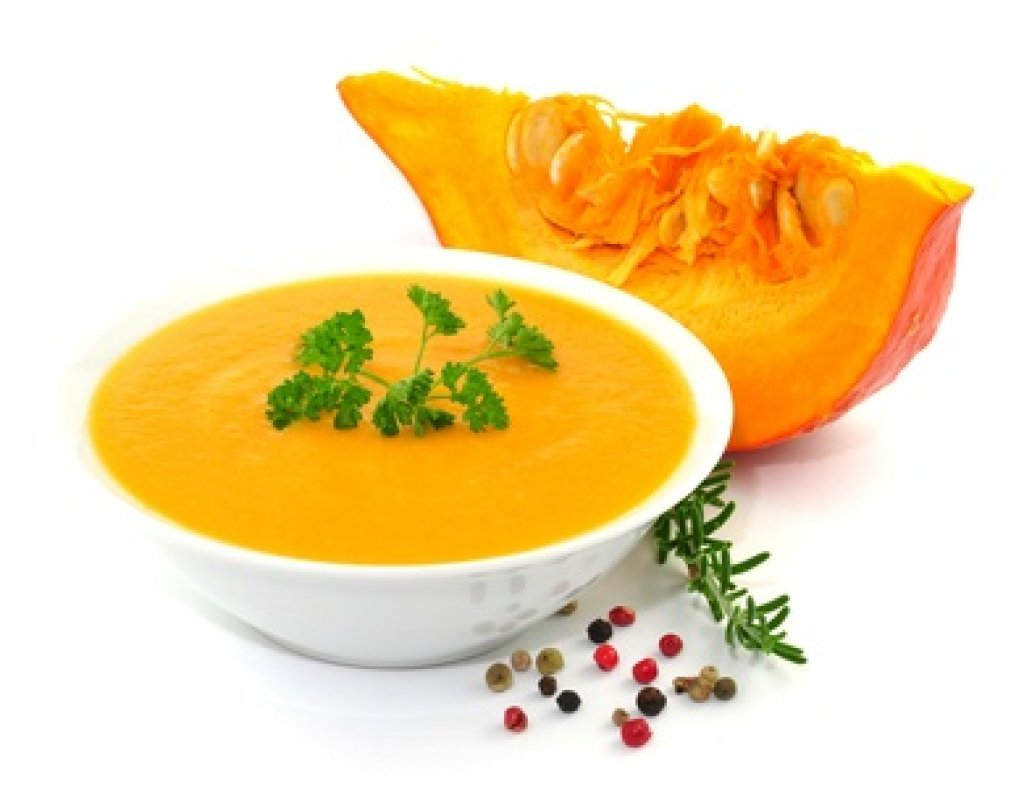
\includegraphics[width=0.35\textwidth]{kuerbissuppe.jpg}
\end{figure}
%Zubereitung:
\begin{Notes}
\item Cut pumpkin into 2\,cm sized dice, carros into slices.
\item Saut\'{e} vegetables for 5\,min in oil, season, add broth and let boil lightly for about  20\,min.
\item Afterward pur\'{e}e.
\end{Notes}
\vfill
\newpage


% Hier steht der Rezepttitel
\section*{K\"{u}rbissuppe}
% Untertitel
\begin{centering}
% Danach die Zutaten in Tabellenform
% Wie viele werden satt?
\end{centering}
%\textbf{Zutaten:}
\begin{table}[H]
\centering
% eine Tabelle mit insgesamt 4 Spalten, falls mehr Zutaten benoetigt werden
% links: Menge, rechts: Zutat
\begin{tabular*}{1\textwidth}{rlrl}
%& && \\
2 & Zwiebeln &&Paprika, edels\"{u}{\ss} \\
600\,g & Hokkaido-K\"{u}rbis & 300\,ml & Orangensaft\\
200\,g & M\"{o}hren & 700\,ml &\ Gem\"{u}sebr\"{u}he \\
2\,El & \"{O}l &&\\
\end{tabular*}
\end{table}
%Zubereitung:
\begin{Notes}
\item Hokkaido in 2\,cm gro{\ss}e W\"{u}rfel schneiden, M\"{o}hren in Scheiben.
\item Gem\"{u}se 5\,min in \"{O}l and\"{u}nsten, w\"{u}rzen, Fl\"{u}ssigkeit
dazugeben und ca. 20\,min k\"{o}cheln lassen.
\item Anschlie{\ss}end p\"{u}rieren.
\end{Notes}
\vfill
\begin{figure}[H]
  \centering
  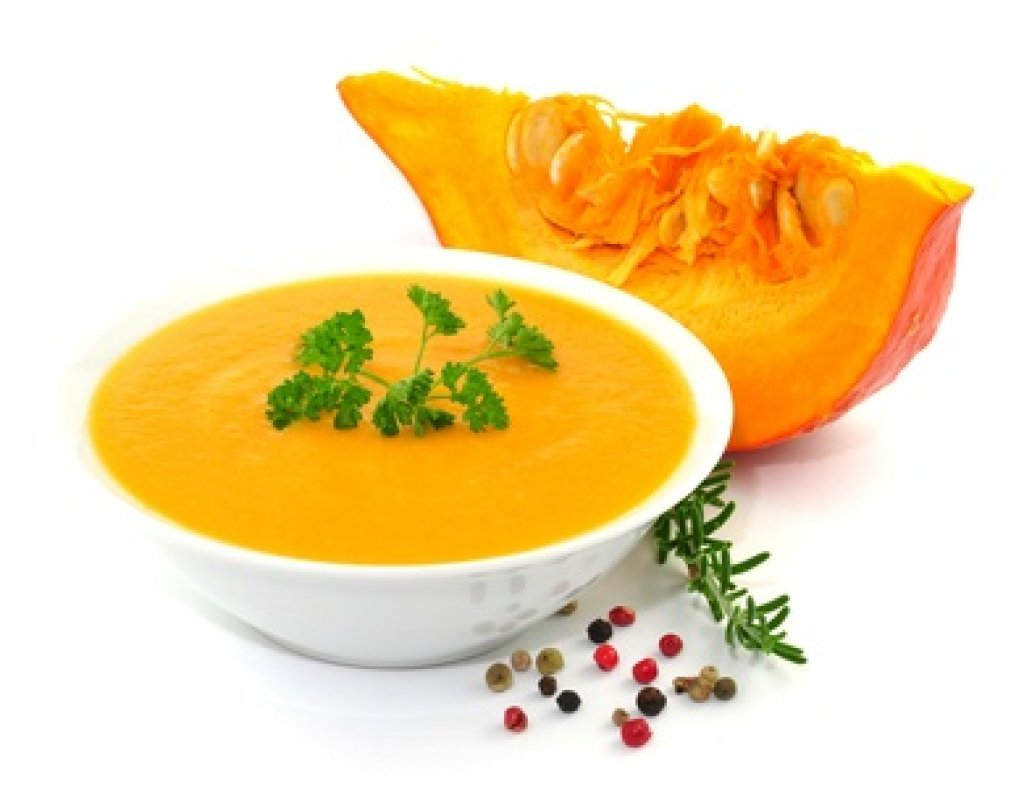
\includegraphics[width=0.75\textwidth]{kuerbissuppe.jpg}
\end{figure}


\newpage
